\documentclass[12pt, oneside]{article}
\usepackage[letterpaper, margin=1in]{geometry}
\usepackage[english]{babel}
\usepackage[utf8]{inputenc}
\usepackage{amsmath}
\usepackage{amsfonts}
\usepackage{amssymb}
\usepackage{tikz}

\usepackage{fancyhdr}
\pagestyle{fancy}
\fancyhf{}
\rhead{Name: \hspace{1.5in} }
\lhead{BECA / Dr. Huson / IB Math SL \\* 1 April 2019\\* 7.8 Do Now: Geometric sequence \& series}

\vspace{1cm}

\renewcommand{\headrulewidth}{0pt}

\title{Worksheet and test template}
\author{Chris Huson}
\date{April 2019}

\begin{document}

\subsubsection*{\\*Geometric sequence and series}

\begin{enumerate}

\item Given a geometric sequence with $u_1=3$ and $r=2.25$
  \begin{enumerate}
      \item Find $u_5$. \\
      (``Find" means you must show the appropriate values substituted into a formula)\\[95pt]
      \item Find $S_5$, the sum of the first five terms of the sequence.\\[145pt]
      \item $S_k=7980$. Find $k$ algebraically.\\[145pt]
      \item Create a table in your calculator to check your answer. (show it to me)
  \end{enumerate}

\newpage
\subsubsection*{Early finishers}

\item Graph $y=400(.85)^{2x}-6$ on the set of axes below.
\begin{center}
    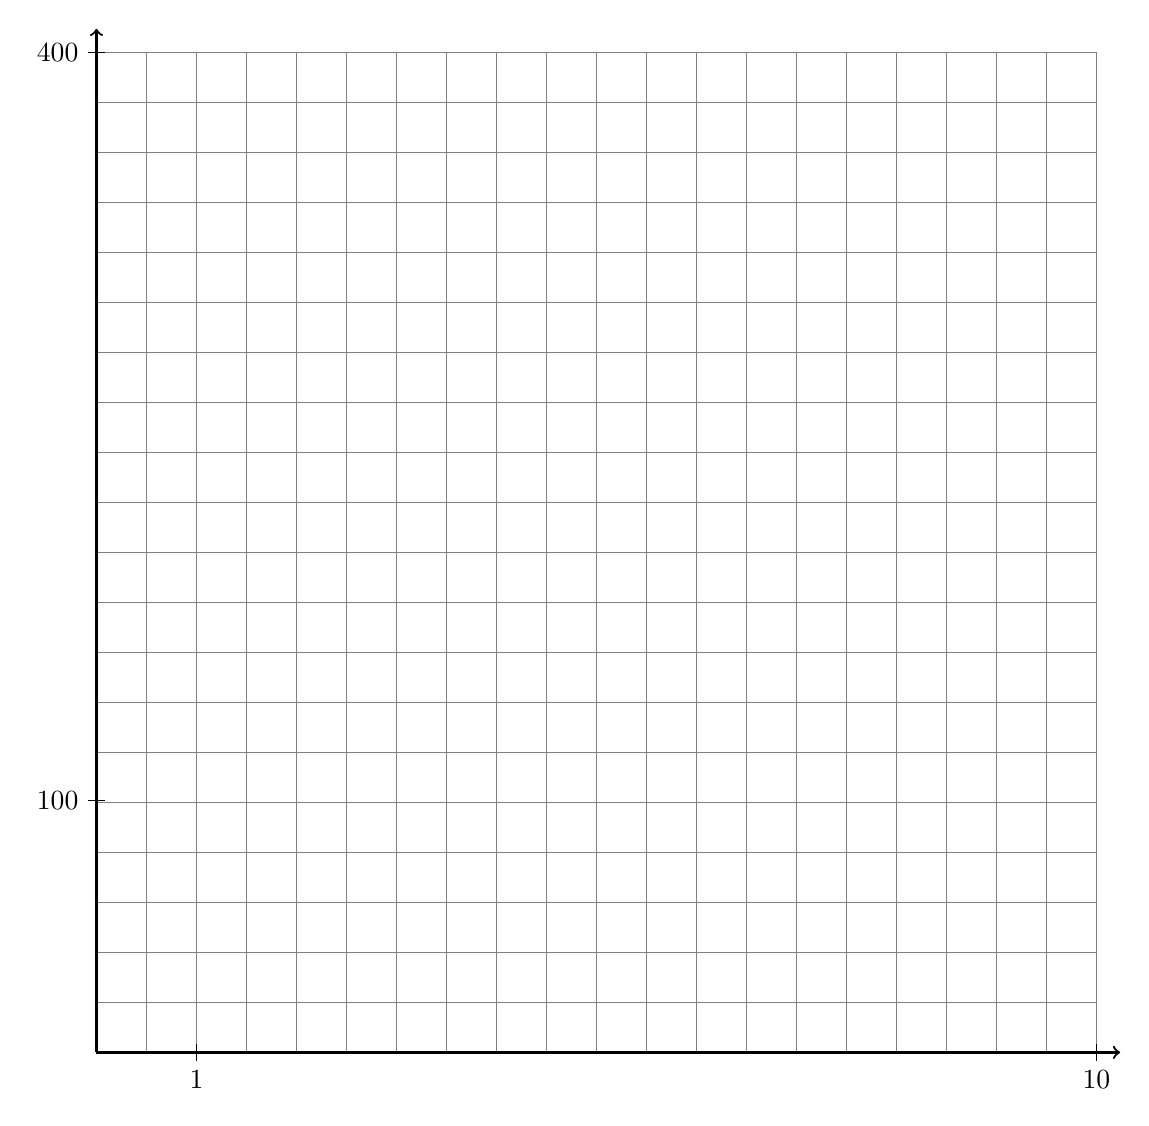
\begin{tikzpicture}
    \draw[step=0.25in,gray,very thin] (0,0) grid (12.7,12.7);
    \draw[thick,->] (0,0) -- (13,0); node[anchor=north west] {x};
    \draw[thick,->] (0,0) -- (0,13); node[anchor=south east] {y};
    \foreach \x in {1.27} \draw (\x cm,3pt) -- (\x cm,-3pt) node[anchor=north] {$1$};
    \foreach \x in {12.7} \draw (\x cm,3pt) -- (\x cm,-3pt) node[anchor=north] {10};
    \foreach \y in {3.2} \draw (3pt,\y cm) -- (-3pt,\y cm) node[anchor=east] {100};
    \foreach \y in {12.7} \draw (3pt,\y cm) -- (-3pt,\y cm) node[anchor=east] {400};
    \end{tikzpicture}
\end{center} %Alg2 Regents Jun2017

\item The expression $(x + a)(x + b)$ can not be written as
\begin{enumerate}
    \item $a(x + b)+ x(x + b)$
    \item $x^2 + (a + b)x + ab$
    \item  $x^2 + abx + ab$
    \item $x(x + a)+ b(x + a)$
\end{enumerate}

\end{enumerate}
\end{document}
